% id: 0344
% book: RPM 중3-2 수학 · 03 원과 직선
% section: 중단원 마무리하기
% figure: crop:fig-0344.png
% answer: ④
% answer_source: 답지
% variant_level: 0 (원본 전사)
% 이 파일은 build.mjs 가 items.json 에서 만든다. 고칠 때는 items.json 을 고친다.
\noindent\begin{minipage}[t]{0.58\linewidth}\vspace{0pt}\raggedright 오른쪽 그림과 같이 두 점~$\pt{A}$, $\pt{B}$는 점~$\pt{P}$에서 원~$\pt{O}$에 그은 두 접선의 접점이다. $\angle\pt{AOB}=120^\circ$, $\seg{OA}=8$일 때, $\seg{AB}$의 길이는?\end{minipage}\hfill\begin{minipage}[t]{0.4\linewidth}\vspace{0pt}\centering \setlength{\dmfigw}{86.9pt}\ifdim\dmfigw>\linewidth\setlength{\dmfigw}{\linewidth}\fi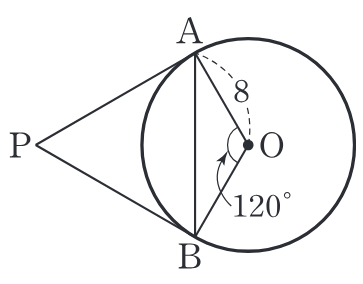
\includegraphics[width=\dmfigw]{figures/fig-0344.png}\end{minipage}\par
\dmchoicesauto{\rule[-3ex]{0pt}{8ex}}{$4\sqrt{3}$}{$6\sqrt{3}$}{$12$}{$8\sqrt{3}$}{$14$}
